
\chapter{ 业务问题所带来的技术挑战@淘宝 }
\thispagestyle{empty}

\setlength{\fboxrule}{0pt}\setlength{\fboxsep}{0cm}
\noindent\shadowbox{
\begin{tcolorbox}[arc=0mm,colback=lightblue,colframe=darkblue,title=学习目标与要求]
%\kai\textcolor{darkblue}{1.~~强化学习.} \\ 

\end{tcolorbox}}
\setlength{\fboxrule}{1pt}\setlength{\fboxsep}{4pt} 

\section{业务问题的思考@淘宝搜索} 

\begin{figure}[h]
\centering
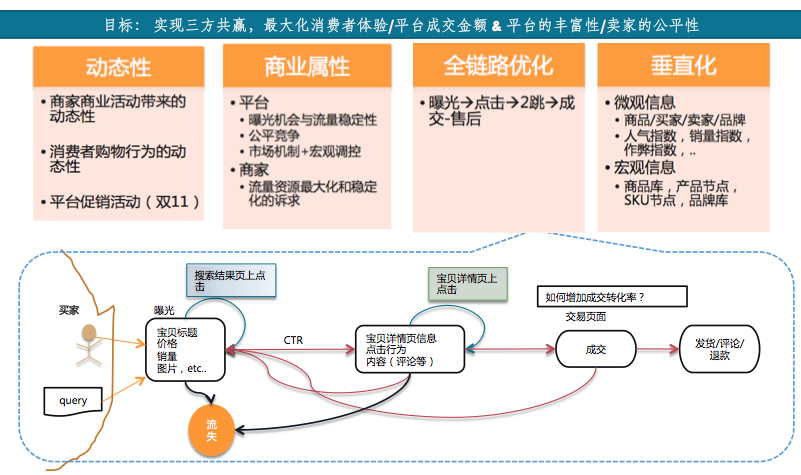
\includegraphics[totalheight=3.0in]{fig/searchProdFea.png}
\caption{电商搜索特性} \label{fig:gansamples}
\end{figure}

淘宝的搜索平台是致力于提供一个一个买家和卖家的公平交易平台;作为一个公平的市场调节员,调整供需平衡,为卖家引导潜在的兴趣用户,以提升其ROI(return on investment),为用户提供满足其需求(user intent)的商品;商业流量下的搜索自然带有其特有的技术特点:

\subsection{动态性}

网页搜索的对象的是分布于各类网站发布的网页,从索引单元上对比,数量上是绝对要远远大于商品搜索的对象集合,如果把每个商品展示页当成是淘宝网站的普通网页的化,表象上讲,商品页面的信息集合应该是网页搜索对象集合的一个子集;网页搜索中的基本对象也存在网页更新,然而淘宝搜索的商品库具有更强的动态性,宝贝的循环搁置,新卖家加入,卖家新商品的推出,价格的调整,标题的更新,旧商品的下架,换季商品的促销,上下架,降价,宝贝图片的更新,销量的变化,卖家等级的提升,商品竞争程度的提升等,都需要淘宝的商品搜索引擎在第一时间捕捉到变化,并及时反映到索引结构中的相应信息单元,而最终的排序环节,这些变化也会动态的融入排序因子,带来排序的动态调整;因此对于商品搜索引擎,要求建立高效的索引更新体系,适应商品类目体系,倒排索引结构,匹配机制的召回逻辑,以及应对商品排序信息及时生效的cache分层机制;

\subsection{全链路优化}

众所周知,相比类似百度这样的网页搜索平台,一个明显的差异是,淘宝搜索平台拥有网购消费者从查询到完成目标商品订单,这样一条完整的行为数据闭合式链路;因此对于用户的一次查询的满意度衡量绝不能止于搜索结果页上看到一个标题相关的商品而发生了点击来判别,post-click之后的商品详情页上的行为,甚至于进入post-pay之后的评论信息都应该成为度量某商品对于某次查询(query)的满意度影响因子;因此,全链路的行为建模会是淘宝搜索体系相比于网页搜索的重要差异之处;既然谈到这点了,再多啰嗦两句,京东也是一家做电子商务的公司,也有着不小的规模,那么如何来看淘宝搜索与京东搜索在全链路优化上的差异呢?从京东模式来看,post-pay环节,由于销售,物流仓储的自营性,可以认为是无差异竞争的;而对于淘宝来说,售后的服务,发货速度,以及纠纷退款等环节是取决于商家与消费者之间的互动来决定的,差异性不言而喻,因此淘宝搜索有必要建立post-pay环节的排序度量因子;

\subsection{商业属性}

电子商务平台的搜索自然具备商业流量的根本属性,商家希望所经营商品通过得到足够的曝光而带来成交;因此,流量资源(曝光)也就成了商家必争之地。搜索排序体系的白盒化和可解释性自然是至关重要。淘宝搜索的ranking,更接近于一个带约束的优化问题,而不是一个简单的排序,优化的目标是最大化平台的成交金额;而约束则是卖家流量分配的诉求;这个环节的涉及到的课题也是电商平台最复杂之处,我会在下面集中阐述下我的一些观点;

\subsection{垂直化}
电子商务搜索属于 vertical search 范畴,相比于网页搜索,对于平台上内容的结构化梳理,以及商业平台上积累的买家,卖家和商品关系数据的挖掘都有更高的要求;因此需要建立 micro analysis 和 macro analysis 双位一体的搜索内容加工体系,宏观分析层面指的是:除了目前已经积累并广泛运用的5级类目之外,完善的商品库建设,spu节点,sku节点,品牌库等,都是必不可少的;微观分析层面则从商品的人气指数,销量指数,作弊指数等角度给出商品自身质量的度量信息;使得搜索结果能够为消费者提供,不仅仅停留在标题相关层面的服务,可以通过合理的宏观分析带来的数据结构化,实现高效的结果查询,通过细致的微观分析,保证优质的商品优先展示给消费者;


\begin{figure}[h]
\centering
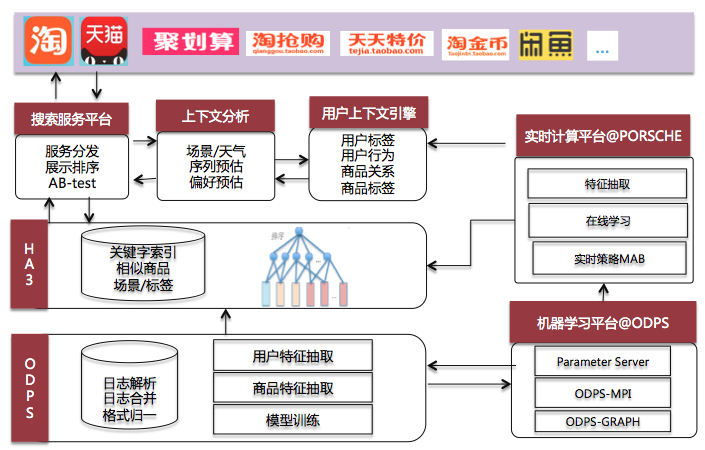
\includegraphics[totalheight=3.0in]{fig/techForBusiness.png}
\caption{智能化助力商业产品} \label{fig:gansamples}
\end{figure}

\section{技术挑战@业务问题} 
\subsection{算法模型} 
像众多互联网企业一样,大数据环境下,基于用户行为建模所面临的技术挑战很多,大家耳熟能详的点列举如下: 
\begin{description}
	\item 投放逻辑带来的数据bias对行为建模的影响
	\item 用户行为数据的稀疏性
	\item 因果关系的模糊性
	\item 用户行为的时效
	\item 行为个性化和非个性化 unified ranking
	\item Cold start modeling
	\item 多样性与精确性的tradeoff (过度个性化)
	\item 长短期个性化融合
\end{description}

\subsection{工程技术} 
随着数据规模的指数级增长,完成复杂数据建模对于工程技术体系的挑战也是不言而喻: 
\begin{description}
	\item 千亿行为和关系数据存储、实时更新和查询
	\item 翻页陷阱
	\item Cache机制
	\item 分级实时体系(数天/小时/秒/ms)
\end{description}

\subsection{效果评估}
效果评估是保证体系迭代朝正向发展的关键保障。
\begin{description}
	\item 模型正确性评估
	\item Ab体系下分群评估
	\item 社会化评测
\end{description} 

\begin{thebibliography}{99}
\addcontentsline{toc}{chapter}{\protect\numberline{}{\hspace{-1.5em}参考文献}}
\markboth{参考文献}{参考文献}
\bibitem{1} C. Burges, T. Shaked, etc.., Learning to rank 
using gradient descent. In Proceedings of the 22nd international 
conference on machine learning, ACM
\end{thebibliography}

 
